\chapter{P\lowercase{riors} O\lowercase{ver} S\lowercase{ampled} S\lowercase{ystems}}

\section{Introduction}
Augmented dynamics provides a flexible way of incorporating useful forms of prior knowledge. However, the most intuitive place to encode such information in a Bayesian framework is directly in the prior distribution over dynamics functions. In fact, augmented dynamics could be viewed as an implication on the covariance matrix or adding additional structure to it. The form of prior knowledge that we address in this chapter is the notion that our discrete-time dynamical system is, in many cases, a sampled continuous-time system. How can we define a prior over discrete-time dynamics that encodes this assumption?

We must first ask, what is the motivation for defining such a prior? What will the likely savings be? In answer to former, we note that it is often the case that the continuous-time dynamics contain some nice structure, for example they can be decomposed as a sum of a linear part, a nonlinear additive part and a general nonlinear part. For example, the pendulum dynamics are made up of a linear and nonlinear part (see \App{pend}) and the cart-pole dynamics consist of a sum of nonlinear combinations of pairs of variables (see \App{cart}). However, this special structure gets lost when we move to the associated discrete-time dynamics. If we were able to encode or learn this underlying structure then our model would be better equipped to generalise into new areas of the state space. In answer to the latter, the likely savings would be that the trained model should have greater marginal likelihood and its predictive performance should be improved with respect to a na\"{\i}ve treatment of the unknown dynamics as a general nonlinear function.

An obvious example of this is, again, time-derivative related states, in which the exact relationship is clear when written in continuous-time but it becomes a complex function of the other (unknown) dynamics, states and actions when dealing in discrete-time. In general any nice structure in the continuous-time dynamics does not translate into the discrete-time domain. It is this problem that we will tackle through the definition of a new class of priors.


%\section{Continuous-Time Implications}
\section{Problem Outline}
In this section we shall address sampled continuous-time systems. These are discrete-time systems which are obtained by sampling some underlying continuous-time system given by
\begin{equation}
\dot\bx_t = \bff(\bx_t, \bu_t)
\label{eqn:conttime}
\end{equation}
where $t \in \RR$. We shall restrict ourselves, as before,  to the consideration of stationary dynamics where $\bff$ is only dependent on $t$ through $\bx$ and $\bu$.  
%
Now assume that $\bff$ has been drawn from some Gaussian process prior $\bff\sim\mathcal{GP}(\bmm, \bK)$. Or in other words
%
\begin{align*}
\bmm(\bz_t) &= \EE_{\bff}\big[\bff(\bz_t)\big] \\
\bK(\bz_t, \tbz_\tau) &= \cov_{\bff}\big[\bff(\bz_t),\bff(\tbz_\tau)\big]
\end{align*}
%
remembering that $\bz := [\bx;\bu]$. This GP prior can encode prior knowledge we have regarding the continuous-time dynamics e.g.\ invariances, linear relationships and additive nonlinear relationships. We are interested in evaluating the associated prior over a sampled version of the dynamics $\bffs\sim\mathcal{GP}(\bmm_\Delta, \bK_\Delta)$ where
%
\begin{align*}
\bmmD(\bz_t) &= \EE_{\bff}\big[\bffs(\bz_t)\big] \\
\bKD(\bz_t,\tbz_\tau) &= \cov_{\bff}\big[\bffs(\bz_t),\bffs(\tbz_\tau)\big]
\end{align*}
%
Note that the expectation and covariance are still taken with respect to the continuous-time dynamics. Now the actual relationship between continuous and the sampled functions is
\begin{align}
\bx_{t+\Dt} &= \bffs(\bx_t,\bu_t) := \bx_t + \int_{t}^{t+\Dt} \!\!\!\!\! \bff(\bx_\tau,\bu_\tau) \dd \tau
\label{eqn:cont-sample}
\end{align}
with sample time $\Dt$. We want to find the relationship between the continuous-time mean and covariance functions ($\bmm,\bK$) and the associated sampled functions ($\bmm_\Delta, \bK_\Delta$). Inevitably we shall have to be satisfied with an approximation since this integral is in general analytically intractable (with the notable exception of linear systems).

In addition, it would be useful to evaluate the posterior GP when we are given non-uniformly sampled data $\cD = \{\bZ,\bY\}$
\begin{align}
\bZ &= \bmat{ \bx_{t_1}\T & \bu_{t_1}\T \\ \vdots & \vdots \\ \bx_{t_n}\T & \bu_{t_n}\T} \in \RR^{n \times D} &\text{and}
&& \bY &= \bmat{ \bx_{t_1+\delta_{1}}\T \\ \vdots \\ \bx_{t_n+\delta_n}\T } \in \RR^{n\times E} \label{eqn:cD}
\end{align}
where the $\delta_i$ can be different. Finally, in order to incorporate it into the predictive framework, moment matching must be possible. We now consider a novel solution to this problem using an approximation based on numerical integration techniques.




% --------------------------------------------------------------------------------------
\begin{table}
\renewcommand{\arraystretch}{1.25}
\begin{center}
\small
\begin{tabular}{ c | ccccc }
\toprule[1.5pt] 
& {\bf Euler } & {\bf Midpoint } & {\bf Heun } & {\bf Kutta } & {\bf RK4 }  \\
\cline{1-6}\\[-2.5ex]
$a_{ip}$
& $\bmat{0}$
& $\bmat{0 & 0 \\ \tfrac{1}{2} & 0}$ 
& $\bmat{0 & 0 \\ 1 & 0}$
& $\bmat{0 & 0 & 0 \\ \tfrac{1}{2} & 0 & 0 \\ -1 & 2 & 0}$
& $\bmat{0 & 0 & 0 & 0 \\  \tfrac{1}{2} & 0 & 0 & 0 \\ 0 & \tfrac{1}{2} & 0 & 0 \\ 0 & 0 & 1 & 0}$ \\[6ex]
$b_{i}$
& $\bmat{1}$
& $\bmat{0 & 1}$ 
& $\bmat{\tfrac{1}{2} & \tfrac{1}{2}}$ 
& $\bmat{\tfrac{1}{6} & \tfrac{2}{3} & \tfrac{1}{6}}$ 
& $\bmat{\tfrac{1}{6} & \tfrac{1}{3} & \tfrac{1}{3} & \tfrac{1}{6}}$  \\[1ex]
\bottomrule[1.5pt]
\end{tabular}
\end{center}
\caption{Settings of $a_{ip}$ and $b_i$ for some common Runge-Kutta methods.}
\label{tab:RKmeths}
\end{table}
% --------------------------------------------------------------------------------------



\section{Numerical Integration}
\subsection{Taylor-Series Expansion}
For clarity of presentation we shall restrict our attention to the autonomous case in which $\dot\bx_t = \bff(\bx_t)$. The full non-autonomous case is addressed in \Sec{nonaut}. One way of dealing with the intractable integral in \Eq{cont-sample} is by expanding out the dynamics function according to its Taylor-series. A first order expansion would yield
\begin{align*}
\bff(\bx_{t+\tau}) &\approx \bff(\bx_t) \;+\; 
\tau \diff{\bff(\bx_{\tilde\tau})}{\tilde\tau}\bigg|_{\tilde\tau=t}  \\[0.1cm]
%
&=  \bff(\bx_t) \;+\; 
\tau \bff_\bx(\bx_t)  \dot\bx_t  \\
&=  \bff(\bx_t) \;+\; 
\tau \bff_\bx(\bx_t) \bff(\bx_t) 
\end{align*}
where $\bff_\bx(\bx_t) := \frac{\dd \bff(\bx)}{\dd \bx}\big|_{\bx=\bx_t} \in \RR^{E\times E}$. The relationship given by \Eq{cont-sample} can then be rewritten as
\begin{equation}
\bffs(\bx_t) \approx \bx_t + 
\Dt \bff(\bx_t) + \tfrac{1}{2}\Dt^2 \bff_\bx(\bx_t) \bff(\bx_t)
\label{eqn:intdt}
\end{equation}
Therefore the approximate relationships between ($\bmm_{\Delta}, \bK_{\Delta}$) and ($\bmm, \bK$) can be characterised by
\begin{align*}
\bmm_{\Delta}(\bx_t) &\approx \bx_t + 
\EE_\bff\big[\Dt \bff(\bx_t) + \tfrac{1}{2}\Dt^2 \bff_\bx(\bx_t) \bff(\bx_t)\big] \\[0.1cm]
%
\bK_{\Delta}(\bx_t,\tbx_\tau) &\approx 
\cov_\bff\big[\Dt \bff(\bx_t) +  \tfrac{1}{2}\Dt^2 \bff_\bx(\bx_t) \bff(\bx_t),\;
\delta_{\tau} \bff(\tbx_\tau) +  \tfrac{1}{2}\delta_{\tau}^2 \bff_\bx(\tbx_\tau) \bff(\tbx_\tau)\big]
\end{align*}
Note that $\Dt$ need not be the same as $\delta_\tau$. There is an issue of prohibitive algebraic complexity, even for this simple approximation. It would involve the calculation of high order moments such as $\cov_\bff\big[\bff_\bx(\bx_t) \bff(\bx_t), \;\bff_\bx(\tbx_\tau) \bff(\tbx_\tau) \big]$ in which it is not clear how this relates to the functions $\bmm$ and $\bK$. Therefore we turn our attention to a widely used and iterative form of numerical integration, the Runge-Kutta (RK) family of methods.





\subsection{Runge-Kutta Methods}
Runge-Kutta methods consist of a simple set of iterative equations which calculate the Taylor-series approximation exactly for a given order $S$. These can be written in the general form
\begin{align}
\bffs(\bx_t) &= \bx_t + \Dt \sum_{i=1}^{S}b_i \bff( \bp_i) \label{eqn:RK1}
\\
\bp_i &= \bx_t + \Dt \sum_{p=1}^{i-1} a_{ip} \bff( \bp_p ) \label{eqn:RK2}
\end{align}
for stationary dynamics where $a_{ip}$, $b_i$ and $c_i$ are the constants associated with a given method. These constants are subject to the constraint $\sum_i b_i = 1$ if the method is to be consistent. By way of example, the constants for some common Runge-Kutta methods are given in \Tab{RKmeths}. These are Euler's method, the Midpoint method, Heun's method, Kutta's method and the popular Runge-Kutta fourth order method (RK4). 
%We shall refer to the family of second order methods as ``RK2", which encompasses both the Midpoint and Heun methods.
Now under this class of methods for numerical integration we can form a tractable approximate relationship from continuous-time to discrete-time as we shall now describe. 




\section{Priors Over Sampled Continuous-Time Systems} \label{sec:priorovercont}


\subsection{Illustrative Examples}
In order to find the relationship between $\bmm$, $\bK$ and $\bmm_{\Delta}$, $\bK_{\Delta}$ consider an approximation using a Runge-Kutta method, given by \Eqs{RK1}{RK2}.
It is useful at this stage to work through the procedure for a couple of simple methods before moving onto the general framework. If we consider the simplest case of an Euler scheme we have the relationship
\begin{align*}
\bffs(\bx) &= \bx + \Dt \bff(\bx)
\end{align*}
It is clear that in this instance the sampled mean and covariance function are simply scalings and translations of the continuous mean and covariance functions
\begin{align*}
\bmm_\Delta(\bx) &= \EE_{\bff}[\bffs(\bx)] &  \bK_\Delta(\bx,\tbx) &= \cov_\bff[\bffs(\bx),\bffs(\tbx)] \\
&= \bx + \Dt \EE_\bff[\bff(\bx)]             & &= \Dt\delta_\tau \cov_{\bff}[\bff(\bx),\bff(\tbx)] \\
&= \bx + \Dt \bmm(\bx)                     & &= \Dt\delta_\tau \bK(\bx,\tbx) 
\end{align*}
Therefore, since the core structure of the sampled mean and covariance remain the same as in continuous-time, we can conclude that \textit{applying the Euler method does not provide any improvement over the standard method in terms of exploiting continuous-time structure}. Now we will work through the Midpoint method, given by
\begin{align*}
\bffs(\bx) &= \bx + \Dt \bff\big(\bx + \tfrac{1}{2}\Dt \bff(\bx)\big)
\end{align*}
First summarise the term in brackets as $\bp = \bx + \tfrac{1}{2}\Dt \bff(\bx)$. It is clear that this will be Gaussian distributed with mean $\bx + \tfrac{1}{2}\Dt \bmm(\bx)$ and covariance $\tfrac{1}{4}\Dt^2 \bK(\bx,\bx)$ for a given value of $\bx$.
%
Therefore the sampled mean and covariance functions will be given by
\begin{align*}
\bmm_\Delta(\bx) &= \bx + \Dt \EE_{\bff,\bp}\big[\bff(\bp)\big]  &  
\bK_\Delta(\bx,\tbx) &= \Dt\delta_\tau\cov_{\bff,\bp,\tbp}\big[\bff(\bp),\bff(\tbp)\big] \\
&= \bx + \Dt \EE_{\bp}[\bmm(\bp)] &
&= \Dt\delta_\tau\Big( \EE_{\bp,\tbp}\big[\bK(\bp,\tbp) + \bmm(\bp)\bmm(\tbp)\T\big] \\[-0.1cm]
&&&\qquad\qquad\qquad\qquad\qquad
-\EE_{\bp}[\bmm(\bp)]\EE_{\tbp}[\bmm(\tbp)]\T \Big)
\end{align*}
where integrals over the continuous mean and covariance function with respect to the random variables $\bp$ and $\tbp$ are required. This is a very similar requirement to the moment matching condition, although now we require cross-covariance terms. The effect of this structural change to the prior will be discussed in \Sec{intuition}. We shall now work through how to do this for a general Runge-Kutta method.


\subsection{General Framework}
Let us employ the assumption that $\bff(\bp_i)$ and $\bff(\tbp_j)$ for $i,j \in \ZZ_{[1,S]}$ are jointly Gaussian distributed given $\bp_i,\tbp_j \sim \cN$. Under this assumption we can apply the process outlined in the illustrative examples for arbitrary orders of the Runge-Kutta method. Note that an implication of this assumption is that $\bp_i$ and $\bp_j$ will be jointly Gaussian since they are related linearly through \Eq{RK2}. In this case we can write
\begin{align}
\bmm_{\Delta}(\bx) &= \bx + \Dt \sum_{i=1}^{S} b_i \,\EE\big[\bff(\bp_i)\big]  \label{eqn:Mdelta} \\
%
\bK_{\Delta}(\bx,\tilde\bx) &= \Dt \delta_{\tau} \sum_{i=1}^{S} \sum_{j=1}^S b_ib_j \,
\cov\big[\bff(\bp_i), \bff(\tbp_j) \big] \label{eqn:Vdelta}
\end{align}
where $\bp_i$ and $\tbp_j$ denote $\bp_i(\bx_t)$ and $\bp_j(\tbx_\tau)$ respectively and the integrals are taken with respect to the random vectors $\bp_i, \tbp_j$ and function $\bff$. 
Similarly for \Eq{RK2} we can use the following iterative rule
\begin{align}
\EE[\bp_i] &= \bx + \Dt \sum_{p=1}^{i-1} a_{ip}\, \EE\big[\bff(\bp_p)\big]
\label{eqn:piter1} \\
\cov[\bp_i, \tbp_j] &= \Dt \delta_{\tau} \sum_{p=1}^{i-1} \sum_{q=1}^{j-1} a_{ip} a_{jq}\, \cov\big[\bff(\bp_p), \bff(\tbp_q)\big]
\label{eqn:piter2}
\end{align}
Now all that remains is to evaluate the expectation $\EE\big[\bff(\bp_i)\big]$ and covariance $\cov\big[\bff(\bp_i), \bff(\tbp_j) \big]$ in these equations. These can be calculated using a moment matching type procedure similar to that of \Sec{multistep}
\begin{align}
\EE_{\bp,\bff}\big[\bff(\bp)\big] 
&= \EE_{\bp}\big[\bmm(\bp)\big] \label{eqn:Efc} \\
\cov_{\bp,\tbp,\bff}\big[\bff(\bp), \bff(\tbp)\big]
&= \EE_{\bp,\tbp}\big[\bK(\bp,\tbp) + \bmm(\bp)\bmm(\tbp)\T\big]
- \EE_{\bp}\big[\bmm(\bp)\big] \EE_{\tbp}\big[\bmm(\tbp)\big]\T \label{eqn:Cfc}
\end{align}
where the integrals are again taken with respect to the random vectors $\bp_i, \tbp_j$ and function $\bff$. The difference between this and the procedure in \Sec{multistep} is that a cross covariance is required in this calculation rather than the covariance of a single random vector $\cov\big[\bff(\bp_i)\big]$. However, any mean and covariance function which satisfies the moment matching criteria will also satisfy this criterion and can be used in this context.

The full structural definition of a new set of priors over sampled autonomous continuous-time dynamical systems is given by \Eqs{Mdelta}{Cfc}. The more general non-autonomous case is discussed in the following section and some examples of kernels for which \Eqs{Efc}{Cfc} can be evaluated are given in \Sec{usekernels}.














\subsection{Non-Autonomous Case} \label{sec:nonaut}
Obviously from a control perspective we are most interested in dealing with systems with external inputs $\bu$. So how do we deal with them in this framework? First imagine that our $\bp$ values are expanded to include a state and an action part $\bp = [\bpx{}; \bpu{}]$. If the action is applied independently of the state over the timestep, for example if it is zero-order hold, first order hold or some other time-dependent function then \Eqs{piter1}{piter2} can be extended trivially as
\begin{align}
\EE[\bp_i] &= \bmat{ \bx \\ \bu + \bee(c_i, \bu) } + \Dt \sum_{p=1}^{i-1} a_{ip}\, 
\bmat{ \EE\big[\bff(\bp_p)\big] \\ \bO } 
\label{eqn:nonaut1} \\
\cov[\bp_i, \tbp_j] &= \Dt \delta_{\tau} \sum_{p=1}^{i-1} \sum_{q=1}^{j-1} a_{ip} a_{jq}\,
\bmat{ \cov\big[\bff(\bp_p), \bff(\tbp_q)\big] & \bO \\ \bO & \bO }
\label{eqn:nonaut2}
\end{align}
where $c_i \in \RR_{[0,1]}$ and $\bee(c_i, \bu) = \bO$ for a zero-order hold scheme and $\bee(c_i, \bu) = c_i(\bu_+ \! - \bu)$, where $\bu_+$ is the action at the following timestep, for a first-order hold scheme. Note that this is not the same as saying that there is not a feedback policy acting on the system, but rather that the policy does not make any state-dependent changes within the sampling window.

Things get a little more complicated if we consider that the action is governed by some policy $\bu = \bpi(\bx)$ over the time interval.  In this case we have the following relationships
\begin{align*}
\EE[\bp_i] &= \bmat{ \bx \\ \bO} + \Dt \sum_{p=1}^{i-1} a_{ip}\, 
\bmat{ \EE\big[\bff(\bp_p)\big] \\[0.1cm] \EE\big[\bpi(\bp_p)\big] }  \\
\cov[\bp_i, \tbp_j] &= \Dt \delta_{\tau} \sum_{p=1}^{i-1} \sum_{q=1}^{j-1} a_{ip} a_{jq}\,
\bmat{ 
\cov\big[\bff(\bp_p), \bff(\tbp_q)\big] & \cov\big[\bff(\bp_p), \bpi(\tbp_q)\big] \\[0.1cm] 
\cov\big[\bpi(\bp_p), \bff(\tbp_q)\big] & \cov\big[\bpi(\bp_p), \bpi(\tbp_q)\big] }
\end{align*}
where the mean $\EE\big[\bpi(\bp_p)\big]$ and covariance $\cov\big[\bpi(\bp_p), \bpi(\tbp_q)\big]$ are dependent only on the form of the function $\bpi$. However, there is no general way of calculating the cross covariance term $\cov\big[\bff(\bp_p), \bpi(\tbp_q)\big]$. Fortunately in this case we can appeal to the results of \Sec{augmentedDYN} to obtain the approximate relationship
\begin{align*}
\cov\big[\bff(\bp_p), \bpi(\tbp_q)\big] &= 
\cov\big[\bff(\bp_p), [\bp_p;\tbp_q] \big]
\cov\big[[\bp_p;\tbp_q]\big]\inv
\cov\big[[\bp_p;\tbp_q], \bpi(\tbp_q)\big]
\end{align*}
to provide a complete framework.





\subsection{Priors Over Useful Function Classes} \label{sec:usekernels}
\subsubsection{Class of Functions}
First we must consider the kind of structure we would like to draw out when we carry out this inference. We believe that a useful space of continuous-time functions to search over is the sum of a full nonlinear part, an additive part and a linear part
\begin{align}
\bff(\bz) &=  \bff_{\text{full}}(\bz) + \bff_{\te{add}}(\bz)  + \bff_{\text{lin}}(\bz)\\
\nonumber &= \bff_{\text{full}}(\bz) + \sum_{i=1}^D\bff_{\te{add},i}\big(z[i]\big) + \bA\bz
\end{align}
If we make the unrestrictive assumption that $\bff_{\text{full}}(\bz)$, $\bff_{\text{add}}(\bz)$ and $\bff_{\text{lin}}(\bz)$ are each drawn from independent Gaussian process priors then the GP parameterising the distribution over the whole function $\bff$ consists simply of the sum of the individual mean and covariance functions
\begin{equation*}
\bff \sim \mathcal{GP}\Big(\bmm_{\text{full}} + \bmm_{\text{add}} + \bmm_{\text{lin}},
\bK_{\text{full}} + \bK_{\text{add}} + \bK_{\text{lin}} \Big)
\end{equation*}
We shall only consider a useful subset of this prior given by $\mathcal{GP}\big(\bmm_{\text{lin}}, \bK_{\text{full}} + \bK_{\te{add}} \big)$.  MATLAB code to evaluate this prior is provided in \App{codePrior} and the function \texttt{prior.m}. We will now evaluate \Eqs{Efc}{Cfc} for each term in this prior.




\subsubsection{Full Nonlinear Part}
A general prior over the space of smooth nonlinear functions is the zero mean, squared exponential covariance prior. In this instance \Eqs{Efc}{Cfc} become 
\begin{align*}
\EE_{\bp,\bff}\big[\bff(\bp)\big] 
&= \mathbf{0} \\
\cov_{\bp,\tbp,\bff}\big[\bff(\bp), \bff(\tbp)\big]
&= \EE_{\bp,\tbp}\big[\bK(\bp,\tbp)\big]
\end{align*}
Again, we shall restrict our attention to a diagonal kernel. The $(a,a)\tth$ element of the expectation of the prior covariance $K[a,a]$ with respect to a joint distribution over the two random variables $\hbp := [\bp;\tbp] \sim \cN(\bm,\bS)$ is then given by
\begin{align}
\nonumber \cov_{\bp,\tbp,\bff}\big[f[a](\bp), f[a](\tbp)\big]
&= \int K[a,a](\hbp) \cN(\hbp | \bm, \bS) \dd \hbp \\
\nonumber &= \int  \alpha_{a}^2 \exp\Big(-\half(\bp - \tbp)\T\bLa_{a}^{-1}(\bp - \tbp) \Big)
\cN(\hbp | \bm, \bS) \dd \hbp \\
\nonumber &= \int  \alpha_{a}^2 \exp\Bigg(-\half\hbp\T 
\underbrace{ \bmat{\bI \\ -\bI}\bLa_{a}^{-1} \bmat{\bI & -\bI} }_{\hat\bLa_{a}^{-1}}
\hbp \Bigg) \cN(\hbp | \bm, \bS) \dd \hbp \\[-0.1cm]
\nonumber &=  \alpha_{a}^2 (2\pi)^{\sfrac{D}{2}}|\hat\bLa_{a}|^{-\sha} \int \cN(\hbp|\bO, \hat\bLa_{a}) \cN(\hbp | \bm, \bS) \dd \hbp \\
&=  \alpha_{a}^2 \big|\bS\hat\bLa_{a}\inv + \bI\big|^{-\sha} 
\exp\Big( - \half \bm\T (\hat\bLa_{a} + \bS)\inv \bm \Big)
\label{eqn:SEprop}
\end{align}
Now since $\hat\bLa_{a}\inv$ is not full rank it should not appear in its un-inverted form. However, we can simply rewrite the term $(\hat\bLa_{a} + \bS)\inv$ as $\hat\bLa_{a}^{-\sha}  \big(\hat\bLa_{a}^{-\sha} \bS\hat\bLa_{a}^{-\sha}  + \bI\big)\inv\hat\bLa_{a}^{-\sha} $ where $\hat\bLa_{a}^{-\sha} = \tfrac{1}{\sqrt{2}}[\bI,-\bI]\T\bLa_{a}^{-\sha}[\bI,-\bI]$ for a numerically stable and symmetric calculation.



\subsubsection{Additive Nonlinear Part}
As shown in \Sec{multistep} the propagation of uncertainty equations for the general additive SE kernel is closely related to the equations for the standard kernel. The same is clearly true in this instance.



\subsubsection{Linear Part}
We have already shown that a distribution of linear systems can be parameterised as
\begin{align*}
\bmm(\bp) &= (\bI \otimes \bp\T)\bet \\
\bK(\bp,\tbp) &= (\bI \otimes \bp\T) \bOm (\bI \otimes \tbp)
\end{align*}
It is clear by looking at the standard moment matching equations provided in \Eqs{linMU}{linSIG} that the expressions for \Eqs{Efc}{Cfc} are very closely related. In fact they are given by
\begin{align*}
\EE_{\bp,\bff}\big[\bff(\bp)\big]  
&= (\bI_E \otimes \mathbf{1}_D\T) \Big( (\mathbf{1}_E  \otimes \bm) \circ \bet \Big) \\
%
\cov_{\bp,\tbp,\bff}\big[\bff(\bp), \bff(\tbp)\big] &= 
 (\bI_E \otimes \mathbf{1}_D\T)
\Big(\big(  \mathbf{1}_{E\times E}\otimes  (\bar\bS + \bm\tilde\bm\T) \big) \big(\bOm+\bet\bet\T\big) \Big) 
 (\bI_E \otimes \mathbf{1}_D) \\[-0.1cm]
& \qquad\qquad\qquad\qquad\qquad\qquad\qquad\qquad\qquad\qquad
- \EE_{\bp,\bff}\big[\bff(\bp)\big] \EE_{\tbp,\bff}\big[\bff(\tbp)\big] \T
\end{align*}
where $\bm = \EE[\bp], \tilde\bm = \EE[\tbp]$ and $\bar\bS = \cov[\bp,\tbp]$. Of course we only require the expression for the mean since we restrict our attention to the prior $\mathcal{GP}\big(\bmm_{\text{lin}}, \bK_{\text{add}} + \bK_{\te{full}} \big)$.







\subsection{Structural Implications on the Prior} \label{sec:intuition}
In order to gain a little more insight into the way the structure of the continuous-time prior is actually altered through this process we shall return to the illustrative example of the midpoint method. We shall consider a uniformly sampled autonomous system with a zero mean squared exponential prior over the continuous-time dynamics. In this case the elements of the sampled mean and covariance functions are
\begin{align}
m_{\Delta}[a](\bx) &= x[a] 
\label{eqn:sampM} \\
K_{\Delta}[a,a](\bx,\tbx) &=
\alpha_{\Delta a}^2
\exp\left(-\half (\bx-\tbx)\T
\bLa_{\Delta a}\inv
(\bx-\tbx) \right)
\label{eqn:sampK}
\end{align}
where $a \in \ZZ_{[1,E]}$. The new output variance $\alpha_{\Delta a}^2$ and length scale terms $\bLa_{\Delta a}\inv$ are functions of the states $\bx$ and $\tbx$. Specifically
\begin{align*}
\alpha_{\Delta a}^2 &=
\Dt^2\alpha_a^2 \left|\tfrac{1}{4}\Dt^2
 \bmat{\bK(\bx,\bx) & \bK(\bx,\tbx) \\ \bK(\tbx,\bx) & \bK(\tbx,\tbx)}
\hat\bLa_{a}\inv + \bI\right|^{-\sha} \\[0.1cm]
%
\bLa_{\Delta a}\inv &=
\half\bLa_{a}^{-\sha} \bmat{\bI & -\bI} \left( \tfrac{1}{4}\Dt^2\hat\bLa_{a}^{-\sha} 
 \bmat{\bK(\bx,\bx) & \bK(\bx,\tbx) \\ \bK(\tbx,\bx) & \bK(\tbx,\tbx)}
\hat\bLa_{a}^{-\sha} + \bI \right)\inv  \bmat{\bI \\ -\bI}\bLa_{a}^{-\sha}
\end{align*}
We can see that the sampled prior in \Eqs{sampM}{sampK} is made up of a linear mean function and a covariance function in the form of a squared exponential but with state-dependant output variance and length-scales. Further, we can see that a cross coupling between the continuous-time hyperparameters has occurred since $\alpha_{\Delta a}$ and $\bLa_{\Delta a}$ are functions of all the hyperparameters in $\bK$, not just $\alpha_a$ and $\bLa_a$.

Finally, we can observe that this prior has the intuitive property that as we let $\Dt \rightarrow 0$ then $\alpha_{\Delta a}^2 \rightarrow \Dt^2\alpha_a^2$ and $\bLa_{\Delta a}\inv \rightarrow \bLa_{a}\inv$. In other words the cross coupling and state dependence of the discrete hyperparameters is turned off as we consider smaller and smaller sampling times.





\subsection{Computational Complexity}
It is important at this stage to include a discussion of the computational complexity of training with this new class of priors. In either case we must first evaluate the prior over the training data parameterised by $\bmm_{\Delta}(\bZ)$ and $\bK_{\Delta}(\bZ,\bZ)$. Clearly $\bK_{\Delta}(\bZ,\bZ)$ is the limiting factor. For the first iteration of any of these methods we are simply calculating the continuous-time prior $\bmm(\bZ)$ and $\bK(\bZ,\bZ)$. This has a complexity of $\cO(En^2)$ for a diagonal covariance function and excluding constant terms. We then need to make $S+\tfrac{1}{2}S(S-1) - 1$ calculations of terms of the form $\EE_{\bP,\tilde\bP}\big[\bK(\bP,\tilde\bP)\big]$ where $\bP, \tilde\bP \in \RR^{n \times D}$. If the continuous-time covariance function is a squared exponential then calculation of this term requires $\cO(D^3En^2)$ since a $2D \times 2D$ matrix needs to be inverted for every pair of data points. If it is a first order additive covariance function then we have complexity of $\cO(DEn^2)$ since we need to carry out $D$ inversions of a $2 \times 2$ matrix for every pair of data points.

In summary, if we include a squared exponential in the covariance function of the continuous-time prior then the evaluation of our discrete-time prior has complexity of the order $\cO(S^2D^3En^2)$ for $S\geq2$ and excluding constant terms. If we do not have a squared exponential but a first order additive squared exponential then this reduces to $\cO(S^2DEn^2)$ for $S\geq2$.










%%%%%%%%%%%%%%%%%%%%%%%%%%%%%%%%%%%%%%%%%%%%





\subsection{Example: Pendulum} \label{sec:pendulum2}
\subsubsection{Inferring Linear Plus Nonlinear Structure}





Recall the pendulum system from \Sec{pendulum} which has the equation of motion
\begin{equation}
\tfrac{1}{3}ml^2 \ddot{\theta} = u - b\dot\theta - \tfrac{1}{2}mlg\sin\theta
\end{equation}
with constants $m=1\!$ kg, $l=1\!$ m, $b = 0.1\!$~N$\,$s$^{-1}$ and $g=9.81\!$~m$\,$s$^{-2}$ from \App{pend}. Initially, we shall consider the unconstrained version of this problem. In continuous-time these dynamics can be decomposed into a linear and a nonlinear part as follows
\begin{align}
\bmat{\dot\theta \\ \ddot\theta} &=
\underbrace{ \bmat{\dot\theta \\ -0.3\dot\theta+3u} }_{\text{Linear}} +
\underbrace{ \bmat{0 \\ -1.5g\sin \theta} }_{\text{Nonlinear}}
\end{align}
The training input data set we considered consisted of $n$ independent samples from the distribution $\bz \sim \cN(\bO,9\bI)$. Although this inference problem looks very simple it is in fact an interesting problem. This is because in continuous-time $\theta$ is given by a simple linear relationship, but in discrete-time this relationship becomes nonlinear as the dynamics get coupled together. It would be useful if our methods could pick out this continuous-time information given the discrete-time data. 

%-------------------------------------------------------------------------------------------------------------------------------------------
\begin{figure}[]
\centering
\small
\begin{tikzpicture}
  \node at (0,0) {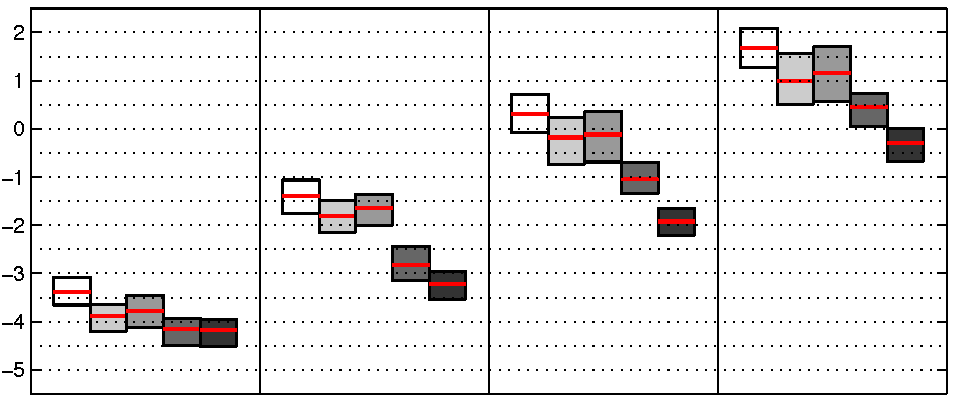
\includegraphics[scale=0.7]{figs/priorcov/plot_nLML.pdf}};
  \draw[rounded corners, fill=white, thick] (6.0,-1.4) rectangle (8.0,1.4); 
  \node[draw, thin, circle, rounded corners, fill=white] at (6,1.0) {}; \node[anchor=west] at (6.3,1.0) {Euler};
  \node[draw, thin, circle, rounded corners, fill=black!20] at (6,0.5) {}; \node[anchor=west] at (6.3,0.5) {Midpoint};
  \node[draw, thin, circle, rounded corners, fill=black!40] at (6,0) {}; \node[anchor=west] at (6.3,0) {Heun};
  \node[draw, thin, circle, rounded corners, fill=black!60] at (6,-0.5) {}; \node[anchor=west] at (6.3,-0.5) {Kutta};
  \node[draw, thin, circle, rounded corners, fill=black!80] at (6,-1.0) {}; \node[anchor=west] at (6.3,-1.0) {RK4};
  \node[rotate=90] at (-6.0,0) {average nLML};
  \node at (-3.9,-2.7) {$\Dt=0.1\,$s};
  \node at (-1.2,-2.7) {$\Dt=0.2\,$s};
  \node at (1.5,-2.7) {$\Dt=0.3\,$s};
  \node at (4.2,-2.7) {$\Dt=0.4\,$s};
\end{tikzpicture}
\caption{Average negative log-marginal likelihoods for discrete GPs with the continuous-time prior $\mathcal{GP}(\bmm_{\text{lin}},\bK_{\text{full}})$ trained on data from the \textit{unconstrained} pendulum. The graph is obtained from 50 Monte-Carlo runs for different types of sampled prior and values of $\Dt$. Each box depicts the 10$\tth$ to 90$\tth$ percentile of the data with the red line showing the 50$\tth$ percentile.}
\label{fig:pend_SEandLIN}
\end{figure}
%-------------------------------------------------------------------------------------------------------------------------------------------



%-------------------------------------------------------------------------------------------------------------------------------------------
\begin{table}[]
\renewcommand{\arraystretch}{1.3}
\begin{center}
\small
%\setlength{\extrarowheight}{2pt}
\rowcolors{3}{black!10}{white}
\begin{tabular}{ cc | ccc | ccc | c }
\toprule[1.5pt] 
&& \multicolumn{3}{c|}{Parameters for $\bmm_{\text{lin}}$}
& \multicolumn{4}{c}{Parameters for $\bK_{\text{full}}$} \\
&& $\eta_{\theta}$ & $\eta_{\dot\theta}$ & $\eta_{u}$ 
& $\lambda_{\theta}$ & $\lambda_{\dot\theta}$ & \multicolumn{1}{c}{ $\lambda_{u}$ } & $\alpha$ \\
\hline
%
Euler & $\theta$ &
0.07  &  {\bf0.95}  &  {\bf0.58}  &  1.38  &  8.26 &  26.25  &  {\bf2.15} \\
 & $\dot\theta$ &
0.41 &  {\bf-0.42}  &  {\bf2.67}  &  1.14  &  {\bf5.55} &  {\bf28.03}  &  9.53 \\
\hline
%
Midpoint & $\theta$ &
0.05 & 0.86 & 0.19 & 1.38 & 61.41 & 44.80 & 0.81 \\
 & $\dot\theta$ &
0.51 & 0.01 & 2.68 & 1.43 & 20.07 & 74.10 & 10.28 \\
\hline
%
Heun & $\theta$ &
0.28 & 0.77 & 0.19 & 3.16 & 54.80 & 79.22 & 1.08 \\
 & $\dot\theta$ &
-0.02 & 0.30 & 2.65 & 1.65 & 15.35 & 102.02 & 13.85 \\
\hline
%
Kutta & $\theta$ &
0.03 & 0.98 & 0.19 & 2.55 & 6.43 & 4.36 & 0.04 \\
& $\dot\theta$ &
0.36 & -0.46 & 2.38 & 1.45 & 176.05 & 39.47 & 11.23 \\
\hline
%
RK4 & $\theta$ &
0.12 & {\bf1.00} & {\bf-0.01} & 0.98 & 3.51 & 3.40 & {\bf0.02} \\
 & $\dot\theta$ &
-0.21 & {\bf-0.54} & {\bf3.06} & 1.39 & {\bf211.30} & {\bf315.35} & 10.13 \\
\bottomrule[1.5pt]
\end{tabular}
\end{center}
\caption{The average of the learned hyperparameters for methods trained using a $\mathcal{GP}(\bmm_{\text{lin}},\bK_{\text{full}})$ continuous-time prior and a setting of $\Dt=0.4\,$s on the \textit{unconstrained} pendulum data. The numbers in bold depict important changes from the Euler to the RK4 method.}
\label{tab:hyps_dt04}
\end{table}
%-------------------------------------------------------------------------------------------------------------------------------------------

%-------------------------------------------------------------------------------------------------------------------------------------------
\begin{table}[t]
\renewcommand{\arraystretch}{1.3}
\begin{center}
\small
%\setlength{\extrarowheight}{2pt}
\rowcolors{3}{black!10}{white}
\begin{tabular}{ cc | ccc | ccc | c }
\toprule[1.5pt] 
&& \multicolumn{3}{c|}{Parameters for $\bmm_{\text{lin}}$}
& \multicolumn{4}{c}{Parameters for $\bK_{\text{full}}$} \\
&& $\eta_{\theta}$ & $\eta_{\dot\theta}$ & $\eta_{u}$ 
& $\lambda_{\theta}$ & $\lambda_{\dot\theta}$ & \multicolumn{1}{c}{ $\lambda_{u}$ } & $\alpha$ \\
\hline
%
Euler & $\theta$ &
0.01 & 0.99 & {\bf0.15} & 1.53 & 90.64 & 140.62 & {\bf0.62} \\
 & $\dot\theta$ &
-0.02 & -0.26 & 2.97 & 1.86 & {\bf21.49} & 233.97 & 14.07 \\
\hline
%
RK4 & $\theta$ &
0.01 & 1.00 & {\bf0.00} & 2.21 & 1.29 & 4.37  &    {$\mathbf{10^{-6}}$} \\
 & $\dot\theta$ &
-0.28 & -0.31 & 3.00 & 1.88 & {\bf421.26} & 429.24 & 13.52 \\
\bottomrule[1.5pt]
\end{tabular}
\end{center}
\caption{The average of the learned hyperparameters for methods trained using a $\mathcal{GP}(\bmm_{\text{lin}},\bK_{\text{full}})$ continuous-time prior and a setting of $\Dt=0.1\,$s on the \textit{unconstrained} pendulum data. The numbers in bold depict important changes from the Euler to the RK4 method.}
\label{tab:hyps_dt01}
\end{table}
%-------------------------------------------------------------------------------------------------------------------------------------------



The first set of simulations was run with a base GP which parameterised a distribution over all linear functions plus a smooth nonlinear part $\bff \sim \mathcal{GP}(\bmm_{\text{lin}},\bK_{\text{full}})$. We sampled 50 different training data sets for various settings of $\Dt$. For each data set we trained the hyperparameters of the different Runge-Kutta based discrete-time priors outlined in the previous section using gradient descent on the average negative Log-Marginal Likelihood (nLML) per data point. The reasoning for the use of this model selection criterion is outlined in \Sec{nLML}. 

This form of prior encodes our knowledge about the form of the continuous-time dynamics and should therefore lead to a significant reduction in the learned nLML. This trend is clearly observed in \Fig{pend_SEandLIN}. As we would expect the saving becomes more significant for larger values of $\Dt$ and the difference in performance between higher order approximations becomes more pronounced. We note that although the Heun and Midpoint methods are both of order two the Midpoint method consistently outperforms the Heun method across all our simulations. The underlying reason for this eludes us.

The average hyperparameters associated with the $\Dt=0.4\,$s runs are given in \Tab{hyps_dt04}. The main parameters responsible for the savings in nLML have been highlighted in bold. Let us first examine the parameters associated with the evolution of $\theta$, shown by the grey rows. We know that in continuous-time the evolution of $\theta$ is given by a purely linear relationship, therefore we would hope that the $\alpha$ parameter in $\bK_{\text{full}}$ would tend to zero. This is the general trend that is in fact observed. We can further note that the linear parameters tend to be closer to the actual continuous-time parameters as the order is increased.

Now we turn our attention to the parameters associated with the evolution of $\dot\theta$. The savings here can be observed by looking at the length-scales $\lambda$ associated with the $\dot\theta$ and $u$ dimensions. Ideally we would like to see these become very large, indicating that the linear component for these dimensions is sufficient to explain the data. Again, this is the trend we can observe. Looking at the linear parameters, we can see that these get closer to the actual values with the exception of the $\dot\theta$ weight. Finally, although the linear parameter for the $\theta$ dimension has not become zero, this is acceptable because it is using this linear part in conjunction with the nonlinearity provided by the SE kernel to explain the sinusoidal relationship.

If we look at the parameters for a setting of $\Dt=0.1\,s$, given in \Tab{hyps_dt01} we can see that the parameters learned by the RK4 method correspond very closely to the idealised relationship. The parameters which lead to the largest savings are again highlighted in bold. Note that the nonlinear term on $\theta$ has been almost completely switched off. For this smaller timestep we can also observe that the crude Euler method has parameters that correspond more closely with our idealised values, as we would expect.




%-------------------------------------------------------------------------------------------------------------------------------------------
\begin{figure}
\centering
\small
\begin{tikzpicture}
  \node at (0,0) {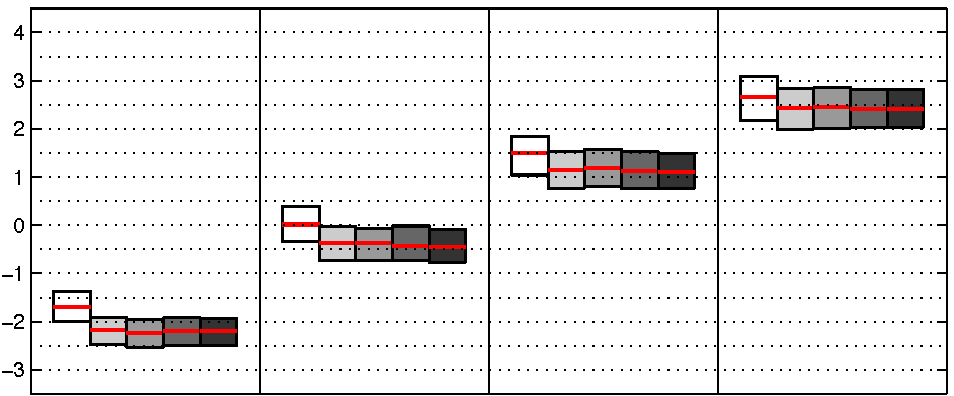
\includegraphics[scale=0.7]{figs/priorcov/plot_nLML_SE.pdf}};
  \draw[rounded corners, fill=white, thick] (6.0,-1.4) rectangle (8.0,1.4); 
  \node[draw, thin, circle, rounded corners, fill=white] at (6,1.0) {}; \node[anchor=west] at (6.3,1.0) {Euler};
  \node[draw, thin, circle, rounded corners, fill=black!20] at (6,0.5) {}; \node[anchor=west] at (6.3,0.5) {Midpoint};
  \node[draw, thin, circle, rounded corners, fill=black!40] at (6,0) {}; \node[anchor=west] at (6.3,0) {Heun};
  \node[draw, thin, circle, rounded corners, fill=black!60] at (6,-0.5) {}; \node[anchor=west] at (6.3,-0.5) {Kutta};
  \node[draw, thin, circle, rounded corners, fill=black!80] at (6,-1.0) {}; \node[anchor=west] at (6.3,-1.0) {RK4};
  \node[rotate=90] at (-6.0,0) {average nLML};
  \node at (-3.9,-2.7) {$\Dt=0.1\,$s};
  \node at (-1.2,-2.7) {$\Dt=0.2\,$s};
  \node at (1.5,-2.7) {$\Dt=0.3\,$s};
  \node at (4.2,-2.7) {$\Dt=0.4\,$s};
\end{tikzpicture}
\caption{Average negative log-marginal likelihoods for discrete GPs with the continuous-time prior $\mathcal{GP}(\bO,\bK_{\text{full}})$ trained on data from the \textit{unconstrained} pendulum. The graph is obtained from 50 Monte-Carlo runs for different types of sampled prior and values of $\Dt$. Each box depicts the 10$\tth$ to 90$\tth$ percentile of the data with the red line showing the 50$\tth$ percentile.}
\label{fig:pend_SEonly}
\end{figure}
%-------------------------------------------------------------------------------------------------------------------------------------------
%-------------------------------------------------------------------------------------------------------------------------------------------
\begin{table}
\renewcommand{\arraystretch}{1.3}
\begin{center}
\small
%\setlength{\extrarowheight}{2pt}
\rowcolors{3}{black!10}{white}
\begin{tabular}{ cc | ccc | c }
\toprule[1.5pt] 
&& \multicolumn{4}{c}{Parameters for $\bK_{\text{full}}$} \\
&& $\lambda_{\theta}$ & $\lambda_{\dot\theta}$ & \multicolumn{1}{c}{ $\lambda_{u}$ } & $\alpha$ \\
\hline
%
Euler & $\theta$ &
{\bf3.97} & 25.31 & 110.29 & 12.26 \\
 & $\dot\theta$ &
2.53 & {\bf37.65} & 31.19 & 43.53 \\
\hline
%
RK4 & $\theta$ &
{\bf288.86} & 90.31 & 307.09 & 59.78 \\
 & $\dot\theta$ &
2.43 & {\bf210.03} & 34.53 & 49.85 \\
\bottomrule[1.5pt]
\end{tabular}
\end{center}
\caption{The average of the learned hyperparameters for methods trained using a $\mathcal{GP}(\bO,\bK_{\text{full}})$ continuous-time prior and a setting of $\Dt=0.1\,$s on the \textit{unconstrained} pendulum data. The numbers in bold depict important changes from the Euler to the RK4 method.}
\label{tab:hyps_SEdt04}
\end{table}
%-------------------------------------------------------------------------------------------------------------------------------------------





The second set of simulations was for a training data set of size $n=30$ but used only a zero-mean GP with a squared-exponential kernel $\bff \sim \mathcal{GP}(\bO,\bK_{\text{full}})$ as a prior over continuous-time dynamics. 
%
The resulting spread in average nLML for a given method and setting of $\Dt$ is depicted in \Fig{pend_SEonly}. It is clear that without prior knowledge of the structure the saving is much less pronounced.


From \Fig{pend_SEonly} we can see that moving from a simple Euler scheme to a higher order method yields a reasonable decrease in nLML. The reason for this saving is clear if we again look at the learned hyperparameters. The average hyperparameters learned over the 50 Monte Carlo runs for $\Dt=0.1\,$s are given in \Tab{hyps_SEdt04} for the Euler and RK4 methods. Only the Euler and RK4 results are given because the values learned for RK4 are not significantly different from those learned for the Midpoint, Heun and Kutta methods. If we observe the numbers highlighted in bold i.e.\ the length-scale associated with $\theta$ and $\dot\theta$ acting on the $\theta$ and $\dot\theta$ state-dimensions respectively then we can see that the higher order methods have assigned these much higher values. In the case of the effect of $\theta$ acting on $\theta$ this is because the RK method has discovered an invariance that was hidden to the simple Euler scheme. Similarly, the higher order RK methods have discovered that the evolution of $\dot\theta$ is in fact only weakly correlated with $\dot\theta$ (a linear scaling of 0.3) and therefore can assign it a long length scale.


The improvement in predictive performance is much less in this case because the algorithm must explain the linear part of the function using only the nonlinear kernel. This means that the only possible saving is from finding invariance or weakly correlated relationships in continuous-time, for example the independence of the rate of change of $\theta$ with respect to $\theta$ itself and the weak correlation of the rate of change of $\dot\theta$ with $\dot\theta$ itself.






Up till now we have been using only the training data set to compare the quality of a given model. We shall now compare the predictive performance on a separate validation data set. To do this we provide a set of $n_v = 50$ data points, again sampled independently from $\bz \sim \cN(\bO,9\bI)$ on which to validate the learned models. Comparison will take place based on two metrics: the \textit{Root Mean Square (RMS) error} and the \textit{negative Log-Predictive Density (nLPD)}. These are given by
\begin{align}
\text{RMS} &= \sqrt{ \frac{1}{n_v} \sum_{i=1}^{n_v} (\bm_i - \bff_{\Delta i})\T(\bm_i - \bff_{\Delta i}) } \\
\text{nLPD} &= \frac{1}{n_v} \left( \sum_{i=1}^{n_v} \tfrac{1}{2}(\bm_i - \bff_{\Delta i})\T\bS_i\inv(\bm_i - \bff_{\Delta i}) 
+ \tfrac{1}{2}\log\big|\bS_i\big| \right) + \tfrac{E}{2}\log(2\pi)
\end{align}
respectively where $\bff_{\Delta i} = \bff_{\Delta}(\bz_i)$ are the underlying function values, $\bm_i = \bmm_{\Delta +}(\bz_i)$ and $\bS_i = \bK_{\Delta +}(\bz_i,\bz_i)$ are the posterior mean and covariance predictions with $\bm_{\Delta +}$ and $\bK_{\Delta +}$ as the posterior sampled mean and covariance functions. We note that although the RMS error is the most commonly used performance measure, it does not take account of the uncertainty measure provided by a Gaussian process. Therefore, we consider the nLPD error to be a more appropriate measure in this probabilistic setting.



%-------------------------------------------------------------------------------------------------------------------------------------------
\begin{figure}
\centering
\footnotesize
\subfigure[Root mean square errors]{
\begin{tikzpicture}
  \node at (0,0) {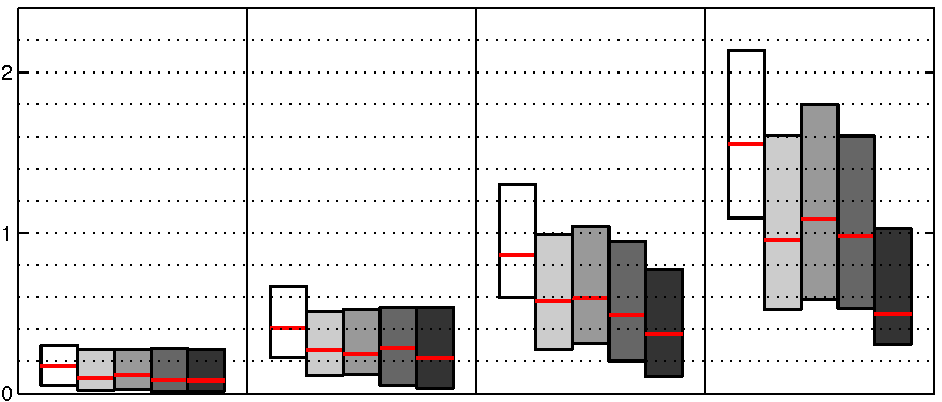
\includegraphics[scale=0.7, clip, trim = 0cm 0cm 0cm 0cm]{figs/priorcov/plot_RMS.pdf}};
  \draw[rounded corners, fill=white, thick] (6.0,-1.4) rectangle (8.0,1.4); 
  \node[draw, thin, circle, rounded corners, fill=white] at (6,1.0) {}; \node[anchor=west] at (6.3,1.0) {Euler};
  \node[draw, thin, circle, rounded corners, fill=black!20] at (6,0.5) {}; \node[anchor=west] at (6.3,0.5) {Midpoint};
  \node[draw, thin, circle, rounded corners, fill=black!40] at (6,0) {}; \node[anchor=west] at (6.3,0) {Heun};
  \node[draw, thin, circle, rounded corners, fill=black!60] at (6,-0.5) {}; \node[anchor=west] at (6.3,-0.5) {Kutta};
  \node[draw, thin, circle, rounded corners, fill=black!80] at (6,-1.0) {}; \node[anchor=west] at (6.3,-1.0) {RK4};
  \node[rotate=90] at (-6.0,0) {RMS};
  \node at (-3.9,-2.7) {$\Dt=0.1\,$s};
  \node at (-1.2,-2.7) {$\Dt=0.2\,$s};
  \node at (1.5,-2.7) {$\Dt=0.3\,$s};
  \node at (4.2,-2.7) {$\Dt=0.4\,$s};
\end{tikzpicture}
}
\subfigure[Negative log-predictive density errors]{
\begin{tikzpicture}
  \node at (0,0) {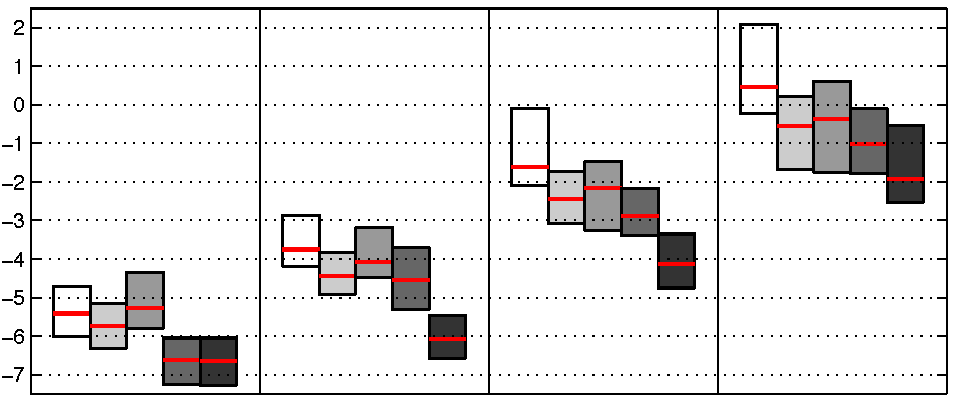
\includegraphics[scale=0.7, clip, trim = 0cm 0cm 0cm 0cm]{figs/priorcov/plot_nLPD.pdf}};
  \draw[rounded corners, fill=white, thick] (6.0,-1.4) rectangle (8.0,1.4); 
  \node[draw, thin, circle, rounded corners, fill=white] at (6,1.0) {}; \node[anchor=west] at (6.3,1.0) {Euler};
  \node[draw, thin, circle, rounded corners, fill=black!20] at (6,0.5) {}; \node[anchor=west] at (6.3,0.5) {Midpoint};
  \node[draw, thin, circle, rounded corners, fill=black!40] at (6,0) {}; \node[anchor=west] at (6.3,0) {Heun};
  \node[draw, thin, circle, rounded corners, fill=black!60] at (6,-0.5) {}; \node[anchor=west] at (6.3,-0.5) {Kutta};
  \node[draw, thin, circle, rounded corners, fill=black!80] at (6,-1.0) {}; \node[anchor=west] at (6.3,-1.0) {RK4};
  \node[rotate=90] at (-6.0,0) {nLPD};
  \node at (-3.9,-2.7) {$\Dt=0.1\,$s};
  \node at (-1.2,-2.7) {$\Dt=0.2\,$s};
  \node at (1.5,-2.7) {$\Dt=0.3\,$s};
  \node at (4.2,-2.7) {$\Dt=0.4\,$s};
\end{tikzpicture}
}
\caption{Comparison of the predictive performance of the RK-based methods given a continuous-time prior $\mathcal{GP}(\bmm_{\text{lin}},\bK_{\text{full}})$ using the RMS and nLPD metrics and based on data from the \textit{unconstrained} pendulum. The graph is obtained from 50 Monte-Carlo runs for different types of sampled prior and values of $\Dt$. Each box depicts the 10$\tth$ to 90$\tth$ percentile of the data with the red line showing the 50$\tth$ percentile.}
\label{fig:pend_validate}
\end{figure}
%-------------------------------------------------------------------------------------------------------------------------------------------




The validation results associated with the previous set of experiments for a continuous-time prior of $\mathcal{GP}(\bmm_{\text{lin}},\bK_{\text{full}})$ are shown in \Fig{pend_validate}. 
%
Across both metrics we can observe that there are substantial improvements in predictive performance as we progress to higher order Runge-Kutta methods and increase $\Dt$. As we move from the Euler to the RK4 method for $\Dt=0.4\,$s we can see that we can get a saving of around a 60\% in the RMS predictive performance.  We note that for this particular problem the improvement in RMS when moving from the Midpoint method to the Kutta method is not significant. However, when compared against the nLPD metric, where the uncertainty prediction is also taken into account, we can observe a reasonable improvement, especially for $\Dt = 0.1\,$s. 
In this particular set of experiments, the Heun method actually performs worse than the Euler method for $\Dt=0.1\,$s with respect to the nLPD. This anomaly could be because the optimisation of the hyperparameters  for the Heun method had not yet converged, or because it had fallen into some local minimum.











\subsubsection{Inferring Linear Plus Additive Structure}
In order to demonstrate the usefulness of the additive kernel, consider a modification to the pendulum equations. Instead of assuming that the input we actually apply is in the range $u\in[-3,3]\,$N we can put this constraint in as another nonlinearity and leave $u$ unconstrained. This leads to the state space equation
\begin{align}
\bmat{\dot\theta \\ \ddot\theta} &=
\underbrace{ \bmat{\dot\theta \\ -0.3\dot\theta} }_{\text{Linear}}  +
\underbrace{ \bmat{0 \\ -1.5g\sin \theta+9\mathrm{sat}(\tfrac{1}{3}u)} }_{\text{Additive}} 
\end{align}
The power of the additive kernel will be in realising that the nonlinearity on $\theta$ and $u$ is linearly separable. This is a ``tighter" space of functions than a completely general nonlinearity over both dimensions.





As before, we obtained a training data set consisting of 30 data points sampled independently from $\bz \sim \cN(\bO,9\bI)$. This is sufficient to excite the ranges of both nonlinear terms. We then trained discrete-time GPs based on a continuous-time prior consisting of linear, additive and full nonlinear terms $\mathcal{GP}(\bmm_{\text{lin}},\bK_{\text{add}} + \bK_{\text{full}})$. The results are shown in \Fig{pend2_SEaSEandLIN}. We can clearly see that the higher order approximations have been able to exploit the underlying structure to produce a model with greater likelihood.  Again, the improvement decreases with the sampling time $\Dt$.





%-------------------------------------------------------------------------------------------------------------------------------------------
\begin{figure}
\centering
\small
\begin{tikzpicture}
  \node at (0,0) {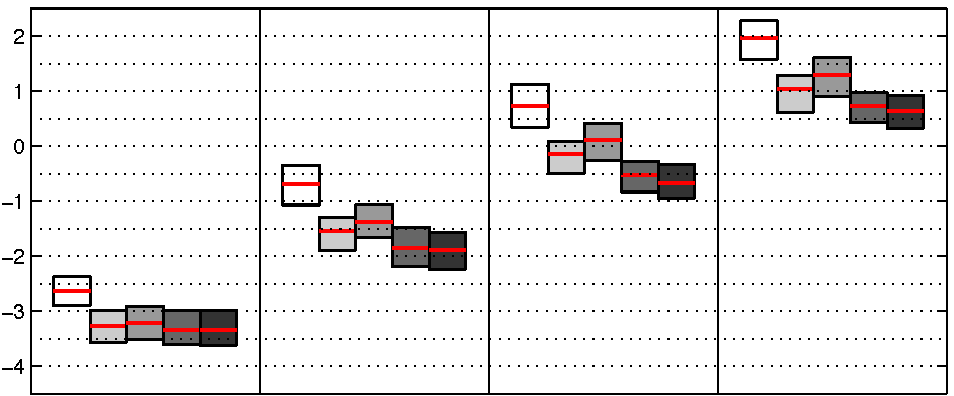
\includegraphics[scale=0.7]{figs/priorcov/plot2_nLML.pdf}};
  \draw[rounded corners, fill=white, thick] (6.0,-1.4) rectangle (8.0,1.4); 
  \node[draw, thin, circle, rounded corners, fill=white] at (6,1.0) {}; \node[anchor=west] at (6.3,1.0) {Euler};
  \node[draw, thin, circle, rounded corners, fill=black!20] at (6,0.5) {}; \node[anchor=west] at (6.3,0.5) {Midpoint};
  \node[draw, thin, circle, rounded corners, fill=black!40] at (6,0) {}; \node[anchor=west] at (6.3,0) {Heun};
  \node[draw, thin, circle, rounded corners, fill=black!60] at (6,-0.5) {}; \node[anchor=west] at (6.3,-0.5) {Kutta};
  \node[draw, thin, circle, rounded corners, fill=black!80] at (6,-1.0) {}; \node[anchor=west] at (6.3,-1.0) {RK4};
  \node[rotate=90] at (-6.0,0) {average nLML};
  \node at (-3.9,-2.7) {$\Dt=0.1\,$s};
  \node at (-1.2,-2.7) {$\Dt=0.2\,$s};
  \node at (1.5,-2.7) {$\Dt=0.3\,$s};
  \node at (4.2,-2.7) {$\Dt=0.4\,$s};
\end{tikzpicture}
\caption{Average negative log-marginal likelihoods for discrete GPs with the continuous-time prior $\mathcal{GP}(\bmm_{\te{lin}},\bK_{\text{add}} + \bK_{\text{full}})$ trained on data from the \textit{artificially constrained} pendulum. The graph is obtained from 50 Monte-Carlo runs for different types of sampled prior and values of $\Dt$. Each box depicts the 10$\tth$ to 90$\tth$ percentile of the data with the red line showing the 50$\tth$ percentile.}
\label{fig:pend2_SEaSEandLIN}
\end{figure}
%-------------------------------------------------------------------------------------------------------------------------------------------
%-------------------------------------------------------------------------------------------------------------------------------------------
\begin{table}
\renewcommand{\arraystretch}{1.3}
\begin{center}
\small
%\setlength{\extrarowheight}{2pt}
\rowcolors{3}{black!10}{white}
\centerline{
\begin{tabular}{ cc | ccc | ccc | ccc | c }
\toprule[1.5pt] 
%&& \multicolumn{3}{c|}{Parameters for $\bmm_{\text{lin}}$}
&& \multicolumn{6}{c|}{Parameters for $\bK_{\text{add}}$} 
& \multicolumn{4}{c}{Parameters for $\bK_{\text{full}}$} \\
%&& $\eta_{\theta}$ & $\eta_{\dot\theta}$ & $\eta_{u}$ 
&& $\lambda_{\theta}$ & $\lambda_{\dot\theta}$ & \multicolumn{1}{c}{ $\lambda_{u}$ }
& $\alpha_{\theta}$ & $\alpha_{\dot\theta}$ & $\alpha_{u}$
& $\lambda_{\theta}$ & $\lambda_{\dot\theta}$ & \multicolumn{1}{c}{ $\lambda_{u}$ } & $\alpha$ \\
\hline
%
Euler & $\theta$ &
1.92 & 7.11 & 2.86 & {\bf0.65} & {\bf0.11} & {\bf0.45} & 1.68 & 9.67 & 71.76 & {\bf1.53} \\
 & $\dot\theta$ &
2.07 & 4.38 & 3.09 & 2.59 & {\bf0.61} & 2.82 & 1.40 & 7.69 & 43.23 & {\bf10.46} \\
\hline
%
RK4 & $\theta$ &
8.93 & 5.40 & 7.81 & {\bf0.18} & {\bf0.008} & {\bf0.05} & 1.03 & 0.81 & 1.78 & {\bf0.005} \\
 & $\dot\theta$ &
1.56 & 2.06 & 2.23 & 10.96 & {\bf0.09} & 2.94 & 1.16 & 1.04 & 3.54 & {\bf0.015} \\
\bottomrule[1.5pt]
\end{tabular}
}
\end{center}
\caption{The average of the learned hyperparameters for methods trained using a $\mathcal{GP}(\bmm_{\text{lin}},\bK_{\text{add}}+\bK_{\text{full}})$ continuous-time prior and a setting of $\Dt=0.3\,$s on the \textit{artificially constrained} pendulum data. The numbers in bold depict important changes from the Euler to the RK4 method.}
\label{tab:hyps2_dt04}
\end{table}
%-------------------------------------------------------------------------------------------------------------------------------------------

%-------------------------------------------------------------------------------------------------------------------------------------------
\begin{figure}
\centering
\footnotesize
\subfigure[Root mean square errors]{
\begin{tikzpicture}
  \node at (0,0) {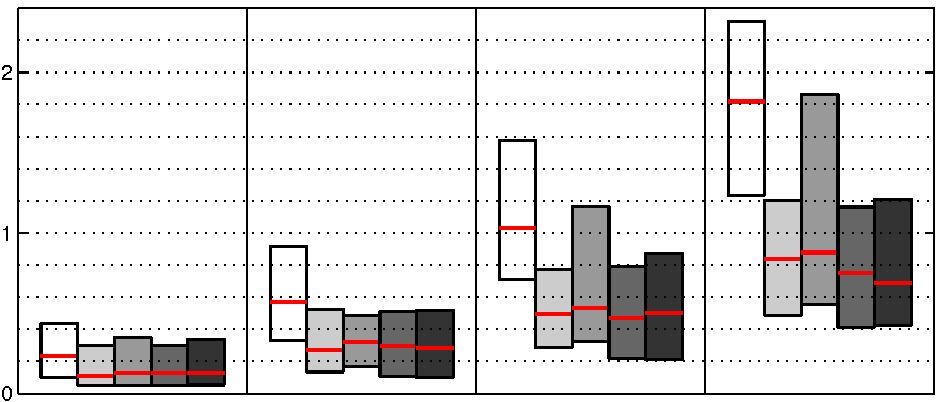
\includegraphics[scale=0.7, clip, trim = 0cm 0cm 0cm 0cm]{figs/priorcov/plot2_RMS.pdf}};
  \draw[rounded corners, fill=white, thick] (6.0,-1.4) rectangle (8.0,1.4); 
  \node[draw, thin, circle, rounded corners, fill=white] at (6,1.0) {}; \node[anchor=west] at (6.3,1.0) {Euler};
  \node[draw, thin, circle, rounded corners, fill=black!20] at (6,0.5) {}; \node[anchor=west] at (6.3,0.5) {Midpoint};
  \node[draw, thin, circle, rounded corners, fill=black!40] at (6,0) {}; \node[anchor=west] at (6.3,0) {Heun};
  \node[draw, thin, circle, rounded corners, fill=black!60] at (6,-0.5) {}; \node[anchor=west] at (6.3,-0.5) {Kutta};
  \node[draw, thin, circle, rounded corners, fill=black!80] at (6,-1.0) {}; \node[anchor=west] at (6.3,-1.0) {RK4};
  \node[rotate=90] at (-6.0,0) {RMS};
  \node at (-3.9,-2.7) {$\Dt=0.1\,$s};
  \node at (-1.2,-2.7) {$\Dt=0.2\,$s};
  \node at (1.5,-2.7) {$\Dt=0.3\,$s};
  \node at (4.2,-2.7) {$\Dt=0.4\,$s};
\end{tikzpicture}
}
\subfigure[Negative log-predictive density errors]{
\begin{tikzpicture}
  \node at (0,0) {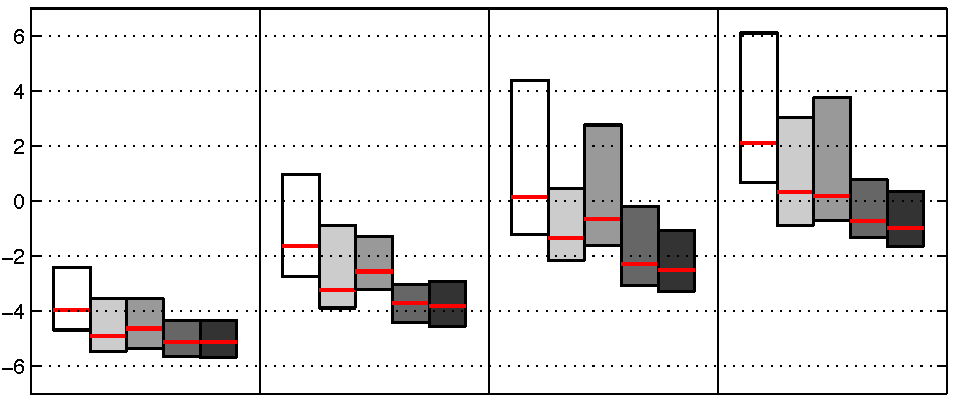
\includegraphics[scale=0.7, clip, trim = 0cm 0cm 0cm 0cm]{figs/priorcov/plot2_nLPD.pdf}};
  \draw[rounded corners, fill=white, thick] (6.0,-1.4) rectangle (8.0,1.4); 
  \node[draw, thin, circle, rounded corners, fill=white] at (6,1.0) {}; \node[anchor=west] at (6.3,1.0) {Euler};
  \node[draw, thin, circle, rounded corners, fill=black!20] at (6,0.5) {}; \node[anchor=west] at (6.3,0.5) {Midpoint};
  \node[draw, thin, circle, rounded corners, fill=black!40] at (6,0) {}; \node[anchor=west] at (6.3,0) {Heun};
  \node[draw, thin, circle, rounded corners, fill=black!60] at (6,-0.5) {}; \node[anchor=west] at (6.3,-0.5) {Kutta};
  \node[draw, thin, circle, rounded corners, fill=black!80] at (6,-1.0) {}; \node[anchor=west] at (6.3,-1.0) {RK4};
  \node[rotate=90] at (-6.0,0) {nLPD};
  \node at (-3.9,-2.7) {$\Dt=0.1\,$s};
  \node at (-1.2,-2.7) {$\Dt=0.2\,$s};
  \node at (1.5,-2.7) {$\Dt=0.3\,$s};
  \node at (4.2,-2.7) {$\Dt=0.4\,$s};
\end{tikzpicture}
}
\caption{Comparison of the predictive performance of the RK-based methods given a continuous-time prior $\mathcal{GP}(\bmm_{\text{lin}},\bK_{\text{add}} + \bK_{\text{full}})$ using the RMS and nLPD metrics and based on data from the \textit{artificially constrained} pendulum. The graph is obtained from 50 Monte-Carlo runs for different types of sampled prior and values of $\Dt$. Each box depicts the 10$\tth$ to 90$\tth$ percentile of the data with the red line showing the 50$\tth$ percentile.}
\label{fig:pend2_validate}
\end{figure}
%-------------------------------------------------------------------------------------------------------------------------------------------





Let us now examine the learned hyperparameters associated with the additive and full nonlinear kernels. These are shown in \Tab{hyps2_dt04} for the Euler and RK4 methods at $\Dt = 0.4\,$s. We can observe where the performance improvement comes from considering the output variance parameters $\alpha$ shown in bold. Ideally we would like to see that the only non-zero terms are the $\alpha_\theta$ and $\alpha_u$ parameters on the $\dot\theta$ dimension. The Euler method has failed to pick up this structure and in fact assigns almost all of the weight to the fully nonlinear term. This is in contrast to the RK4 method which assigns nothing to the general nonlinearity and removes the irrelevant terms from the additive part.


Finally, we compare the predictive performance of these methods given a validation data set of 50 points with inputs sampled from $\bz \sim \cN(\bO,9\bI)$ as before. The results are shown in \Fig{pend2_validate}. In terms of RMS error we can observe a significant improvement from the Euler to the Midpoint and Heun methods, but not much further improvement beyond that. However, if we compare under the negative log-predictive likelihood we see that the higher order methods do in fact provide a significant improvement based on their estimate of the predictive uncertainty.







%\section{Additive Structure}
%\subsection{Overview}
%Often, it will be clear from some prior first principles knowledge, or otherwise, that the dynamics of a given system are not made up of arbitrary nonlinear interactions between states and actions but a sum of lower order interactions. For example, the case where the function is purely additive
%\begin{equation}
%\bff(\bz) = \sum_{d=1}^D \bff_i\big(z^{(d)}\big)
%\end{equation}
%If each function $\bff_d$ is assumed to be a priori independent of each other and each is assumed to be drawn from a 1-D GP $\bff_d \sim \mathcal{GP}(\bmm_d,\bK_d)$ then the structure of the mean and covariance functions of the full function $\bff \sim \mathcal{GP}(\bmm,\bK)$ is clearly
%\begin{align}
%\bmm(\bz) &= \sum_{d=1}^D \bmm_i\big(z^{(d)}\big) \\
%\bK(\bz,\tbz) &= \sum_{d=1}^D \bK_i\big(z^{(d)}, \tilde z^{(d)}\big)
%\end{align}
%Since this effectively reduces the space of functions under consideration, learning may proceed more effectively.
%One could equally consider higher order interactions such as
%\begin{equation}
%\bff(\bz) = \sum_{d=1}^D \bff_d\big(z^{(d)}\big)
%+ \sum_{d=1}^D\sum_{e=d+1}^D \bff_{de}\big(z^{(d)}, z^{(e)}\big) + \dots
%\end{equation}
%with similar implications on the mean and covariance functions of the full function. Additive GPs of arbitrary order with squared exponential base-kernels are considered in \cite{DNR11}. A useful trick is applied in this paper, making use of the Newton-Girard formulae, such that evaluation of the full additive kernel (the sum over all possible interactions) does not grow exponentially as $\mathcal{O}(2^E)$ but as $\mathcal{O}(D^2)$. Regrettably this trick does not apply when propagating uncertainty through predictions as will be shown in the following section.
%Other forms of structure could also be incorporated, for example, the case in which the dynamics are affine in the action $\bu$
%\begin{equation}
%\bff(\bz) = \bff_{\bx}(\bx) + \sum_{f=1}^F \bff_f(\bx) u^{(f)}
%\end{equation}
%which would lead to a mean and covariance function of the form
%\begin{align}
%\bmm(\bz) &= \bmm_{\bx}(\bx) + \sum_{f=1}^F \bmm_f(\bx) u^{(f)} \\
%\bK(\bz,\tbz) &= \bK_{\bx}(\bx,\tilde\bx) + \sum_{f=1}^F \bK_f(\bx,\tilde\bx) u^{(f)} u^{(f)}
%\end{align}






\section{Combining Time-Derivative and Sampled Data}
\subsection{Single Data Points}

Now let us suppose that we actually have access to samples of states, actions and time derivatives of the states themselves. In other words our data set now has the form
\begin{align}
\bZ &= \bmat{ 
\bx_{t_1}\T & \bu_{t_1}\T \\ \vdots & \vdots \\ 
\bx_{t_m}\T & \bu_{t_m}\T \\[0.1cm]
\bx_{t'_{1}}\T & \bu_{t'_{1}}\T \\ \vdots & \vdots \\ 
\bx_{t'_n}\T & \bu_{t'_n}\T} \in \RR^{(m+n) \times D} &\text{and}
%
&& \bY &= \bmat{ 
\dot\bx_{t_1}\T \\ \vdots \\ 
\dot\bx_{t_m}\T \\[0.1cm] 
\bx_{t'_{1} + \delta_{1}}\T \\ \vdots \\ 
\bx_{t'_n + \delta_n}\T} \in \RR^{(m+n)\times E} \label{eqn:cDD}
\end{align}
%
It would be ideal if we could use the whole data set for training and prediction with our Gaussian process. But how do we combine these two kinds of data? Since we already have a means of evaluating continuous data (using the specified continuous GP) and sampled data (using the RK-based method from \Sec{priorovercont}) the only thing we need to derive is the cross covariance term $\bK_{\times}(\bz_t,\tilde\bz_\tau) := \cov_{\bff}[\bffs(\bz_t),\bff(\tbz_\tau)]$. It is clear from the equations we derived in \Sec{priorovercont} that this will be equal to
\begin{align}
\bK_{\times}(\bz_t,\tilde\bz_\tau) &= \Dt \sum_{i=1}^{S} b_i \,
\cov_{\bp_i,\bff}\big[\bff(\bp_i), \bff(\tbz_\tau) \big]
\label{eqn:lalalala}
\end{align}
given a certain RK scheme. The covariance term in this equation can be calculated using a simplification of the equations derived in \Sec{usekernels} where the distribution is only over the first argument $\bp_i$. The distribution over $\bp_i$ can be found using \Eqs{piter1}{piter2} by setting $\tbp_j = \bp_i$. In the non-autonomous case \Eqs{nonaut1}{nonaut2} should be used. 


\subsection{State-Action Derivative Observations}

\subsubsection{Overview}
It was observed by \cite{SMLL03} that the derivative of a Gaussian process remains a Gaussian process. This means that we can combine not only observed points from our unknown function but also gradient observations. In fact this notion can be generalised to any linear operation and is presented in its general form by \cite{Sar11}. We shall restrict our attention to gradient observations since this is the most useful in the context of dynamical systems.

The incorporation of local linear models as derivative models in a Gaussian process modelling framework for dynamical systems is not a new concept. They have been used for system identification by \cite{AK11} and in a model predictive control framework by \cite{AK08}. These papers consider only ARX models, where the system has a single output and input and the state is made up of lagged versions of these. The work of this thesis extends the use of derivative observations to general state-spaces and to the incorporation of known continuous-time linear models.

\subsubsection{General Kernels}
The covariances between a pair of data points and the associated derivatives are simply given by the corresponding derivatives of the covariance function itself
\begin{align*}
\cov_{\bff}\Big[\bff(\bz), \bff(\tilde\bz)\Big] &= \bK(\bz,\tilde\bz) \\
\cov_{\bff}\Bigg[\pdiff{\bff(\bs)}{s[i]}\bigg|_{\bs = \bz}, \bff(\tilde\bz) \Bigg] 
&= \bK^i(\bz,\tilde\bz) := \pdiff{\bK(\bs,\tilde\bz)}{s[i]}\bigg|_{\bs = \bz} \\[0.1cm]
\cov_{\bff}\Bigg[\pdiff{\bff(\bs)}{s[i]}\bigg|_{\bs = \bz}, \pdiff{\bff(\tbs)}{\tilde s[j]}\bigg|_{\tbs = \tbz} \Bigg] 
&= \bK^{i,j}(\bz,\tilde\bz) := \pdiff{^2\bK(\bs,\tbs)}{s[i]\partial \tilde s[j]}\bigg|_{\bs = \bz,\tbs = \tbz}
\end{align*}
From these definitions we can also define the block matrices
\begin{equation*}
\bK'(\bz,\tbz) := \bmat{\bK^1(\bz,\tilde\bz) \\ \vdots \\ \bK^D(\bz,\tilde\bz)} 
\quad \text{and} \quad
\bK''(\bz,\tbz) := \bmat{\bK^{1,1}(\bz,\tilde\bz) & \dots & \bK^{1,D}(\bz,\tilde\bz) \\ 
\vdots & \ddots & \vdots \\ \bK^{D,1}(\bz,\tilde\bz) & \dots & \bK^{D,D}(\bz,\tilde\bz)} 
\end{equation*}
The final piece of information we need in order to use it as a base kernel for our sampled continuous-time prior is to find the expectations $\EE_{\bp,\tbp}\big[\bK'_i(\bp,\tbp)\big]$ and $\EE_{\bp,\tbp}\big[\bK''_{ij}(\bp,\tbp)\big]$ for $\hbp := [\bp;\tbp] \sim \cN(\bm,\bS)$.


\subsubsection{Squared Exponential Kernel}
As usual, we shall restrict our attention to a diagonal kernel where the $(a,a)\tth$ element of the prior covariance is $k_a := K[a,a]$. The expressions for $k'_a(\bz,\tbz)$ and $k''_a(\bz,\tbz)$ in this case are
\begin{align*}
k'_a(\bz, \tilde\bz) &= - k_a(\bz,\tilde\bz) \bLa_a\inv (\bz - \tbz) \\
k''_a(\bz, \tilde\bz) &= k_a(\bz, \tilde\bz)  \Big(\bLa_a\inv
- \bLa_a\inv (\bz - \tbz)(\bz - \tbz)\T \bLa_a\inv \Big) 
\end{align*}
By defining $\hbz := [\bz; \tbz]$ we can rewrite these equations in the form
\begin{align*}
k'_a(\hbz) &= - k_a(\hbz) \bLa_a\inv \bmat{\bI & - \bI} \hbz \\
k''_a(\hbz) &= k_a(\hbz)  \bigg(\bLa_a\inv
- \bLa_a\inv \bmat{\bI & - \bI} \hbz\hbz\T\bmat{\bI \\ - \bI} \bLa_a\inv \bigg) 
\end{align*}
This will help us in evaluating the expectation of the first expression
\begin{align}
\nonumber \EE_{\bp,\tbp}\big[k'_a(\bp,\tbp)\big]
&= -  \bLa_a\inv  \int \bmat{\bI & -\bI}\hbp k_a(\hbp) \cN(\hbp | \bm, \bS) \dd \hbp \\
%
\nonumber &=  - \alpha_{a}^2 (2\pi)^{D/2}|\hat\bLa_{a}|^{1/2} \bLa_a\inv \bmat{\bI & -\bI}
\int \hbp \cN(\hbp|\bO, \hat\bLa_{a}) \cN(\hbp | \bm, \bS) \dd \hbp \\
%
%\nonumber &=  \alpha_{a}^2 \big|\bS\hat\bLa_{a}\inv + \bI\big|^{-1/2} 
%\exp\Big( - \half \bm\T (\hat\bLa_{a} + \bS)\inv \bm \Big)
%\bS(\hat\bLa_a+\bS)\inv \bm \\
&= - \EE_{\bp,\tbp}\big[k_a(\bp,\tbp)\big]  \bLa_a\inv \bmat{\bI & -\bI} \hat\bm
\end{align}
where $\hat\bm := \bS(\hat\bLa_a+\bS)\inv\bm$. The first step is achieved by noting the similarity with \Eq{SEprop} and the second using the identity for the multiplication of two Gaussian densities given in \App{gauss}. We reiterate from our discussion of \Eq{SEprop} that the term $(\hat\bLa_{a} + \bS)\inv$ can be calculated in a numerically stable manner as $\bLa_a\inv(\bS\hat\bLa_{a}\inv + \bI)\inv$. Now turning our attention to the second integral we get
\begin{align}
\nonumber \EE_{\bp,\tbp}\big[k''_a(\bp,\tbp)\big]
&= \bLa_a\inv  \int k_a(\hbp) \cN(\hbp | \bm, \bS) \dd \hbp \\[-0.2cm]
\nonumber& \qquad\qquad\qquad\qquad
- \bLa_a\inv \bmat{\bI & -\bI} \int \hbp\hbp\T k_a(\hbp) \cN(\hbp | \bm, \bS) \dd \hbp \bmat{\bI \\ -\bI} \bLa_a\inv \\
%
&=    \EE_{\bp,\tbp}\big[k_a(\bp,\tbp)\big] \Bigg(
 \bLa_a\inv - \bLa_a\inv \bmat{\bI & -\bI} \Big(
\hat\bS + \hat\bm \hat\bm\T
\Big)\bmat{\bI \\ -\bI} \bLa_a\inv 
\Bigg)
\end{align}
where $\hat\bS := \hat\bLa_a(\hat\bLa_a+\bS)\inv\bS$ is obtained from the results in \App{gauss}. Again, we can write this term as $(\bS\hat\bLa\inv_a + \bI)\inv\bS$ for a numerically stable calculation.


\subsubsection{Additive Squared Exponential Kernel}
The derivation of these equations is again closely related to the squared exponential and can be obtained by following a similar procedure to \Sec{multistep}.



\subsection{Local Model Validation}
The framework outlined in the previous section can be used to validate a given continuous-time local linear model given sampled observations. First, consider a local linear model of the form
\begin{equation*}
\dot\bx = \bo_{\text{m}} + \bW(\bz - \bz_{\text{m}})
\end{equation*}
based around the operating point $\bz_{\text{m}}$ where the offset term $\bo_{\text{m}}$ is zero if $\bz_{\text{m}}$ is an equilibrium of the system. We could create an artificial data set $\cD = \{\bZ_{\text{m}},\bY_{\text{m}}\}$ defined by
\begin{equation*}
\bZ_{\text{m}} = \bmat{\bar\bz\T \\ \bar\bz\T \otimes \mathbf{1}_D} \in \RR^{(D+1)\times D}
\quad\text{and}\quad
\bY_{\text{m}} = \bmat{\bar\bo\T \\ \bW\T} \in \RR^{(D+1)\times E}
\end{equation*}
The framework outlined in the previous section then allows us to calculate the joint prior distribution with a standard data set
\begin{equation*}
\left.\bmat{\vec\bY_{\text{m}} \\ \vec\bY} \right| \bZ_{\text{m}}, \bZ, \hyp  \sim \cN\left(
\bmat{ \bmm(\bZ_{\text{m}}) \\ \bmm(\bZ) },
\bmat{\bK(\bZ_{\text{m}},\bZ_{\text{m}})+ c_{\text{m}}\inv \bI & \bK(\bZ_{\text{m}},\bZ) \\ 
\bK(\bZ,\bZ_{\text{m}}) & \bK(\bZ,\bZ) + \bS_{\be} \otimes \bI }
\right)
\end{equation*}
where $\bmm$ and $\bK$ apply the appropriate operations described in the previous sections. The key thing to note here is the introduction of a ``confidence" parameter $c_{\text{m}}$ which we can consider as an additional parameter appended to the hyperparameter vector $\hyp$. Whilst training, this parameter can be automatically tuned through maximisation of the marginal likelihood as described in \Sec{nLML}. The learned parameter will then reflect how well the given local model agrees with the observed data. For example, if $c_{\text{m}} \rightarrow 0$ the training process has determined that the given model does not agree with the data. Conversely, if $c_{\text{m}}$ becomes very large, the given model closely agrees with the data.








\section{Summary}
We have defined a new class of Gaussian process priors for sampled continuous-time systems. The problem we were addressing was how we could exploit useful structure in the continuous-time dynamics of a system in which we only have access to sampled data and must make predictions in discrete-time. In particular, we wanted to exploit this structure for training models with greater marginal likelihood and improved predictive performance. We achieved this objective by finding an approximate relationship, based on the Runge-Kutta family of methods, between a Gaussian process prior placed over the continuous dynamics and the associated prior over the sampled system. 


The effectiveness of this method was demonstrated on data sets obtained from the pendulum system. The continuous-time pendulum dynamics can be decomposed into a linear part plus an (additive) nonlinear part. We showed that a standard discrete-time prior often failed to pick out this structure and the invariances in the equations. On the other hand, our Runge-Kutta class of priors were able to learn hyperparameters that corresponded very closely to the underlying continuous-time structure, which led to models with greater marginal likelihood than the standard method. As we would expect, this improvement increased with the order of the RK method being utilised, but at the expense of increased computational load. We observed improvement not only in the marginal likelihood of the model but also in terms of predictive performance.


The class of priors we have defined can additionaly handle non-uniformly sampled data sets and data sets with mixtures of continuous and sampled data. This may be especially useful in the case where we would like to test how well a given continuous local-linear model of a system agrees with the observed sampled data. We ended by designing an algorithm to achieve such a test and to return a parameter which puts a numerical value on how well a given local model agrees with the observed data.


